%%%%%%%%%%%%%%%%%%%%%%%%%%%%%%%%%%%%%%%%%%%%%%%%%%%%%%%%%%%%%%%%%%%%%%%%%%%%%%%%
\chapter{Future Work}
%%%%%%%%%%%%%%%%%%%%%%%%%%%%%%%%%%%%%%%%%%%%%%%%%%%%%%%%%%%%%%%%%%%%%%%%%%%%%%%%
\label{sec:future}

As Landslide is an experimental foray into the world of systematic exploration in kernel-space, and a detailed study of systematic exploration in general, it has opened up many avenues for potential future improvements.

%%%%%%%%%%%%%%%%%%%%%%%%%%%%%%%%%%%%%%%%%%%%%%%%%%%%%%%%%%%%%%%%%%%%%%%%%%%%%%%%
\section{Interface Improvements}
\label{sec:future-interface}

In Section~\ref{sec:eval-feedback}, we describe many ways in which Landslide's user interface is lacking. These improvements would not necessarily be research developments, but would enhance the user experience in ways necessary for continuing work in the context of 15-410.\footnote{
Landslide is also missing functionality to automatically identify decision points when newly-forked threads become runnable but not immediately switched to. This was not necessary to find the \texttt{double\_thread\_fork} bug in POBBLES (Section~\ref{sec:eval-casestudy}) only because POBBLES automatically switched to the child thread immediately.}

\begin{itemize}
	\item Landslide currently does not support ability to replay a particular choice sequence. If the user finds a bug, and wants to re-execute the interleaving that led to it, they have no choice but to re-explore the tree.
	\item Although Simics can pause execution and give the user a debug prompt, Landslide currently does not support being interrupted during exploration.
		This is because the current implementation uses a wrapper script around the Simics prompt which Landslide communicates with to perform backtracking.
		Though it would be difficult to redesign, it would be good to work around, to enable the user to interrupt, use the Simics debug prompt arbitrarily, and resume Landslide when ready.
	\item Landslide could print its decision traces in a better format. The current format is basically a ``raw data dump''. Raw text is probably the wrong interface; a graphical/tabular format with distinct columns for the execution of each different thread would be easier to understand.
	\item Landslide could attempt to detect when something has gone wrong that is not its fault (such as incorrect instrumentation, or the kernel violating some of its requirements), and print a useful error message rather than behaving mysteriously.
\end{itemize}

%%%%%%%%%%%%%%%%%%%%%%%%%%%%%%%%%%%%%%%%%%%%%%%%%%%%%%%%%%%%%%%%%%%%%%%%%%%%%%%%
\section{Education}
\label{sec:future-education}

\subsection{Landslide as a Teaching Tool}

\begin{figure*}[h]
	\begin{center}
	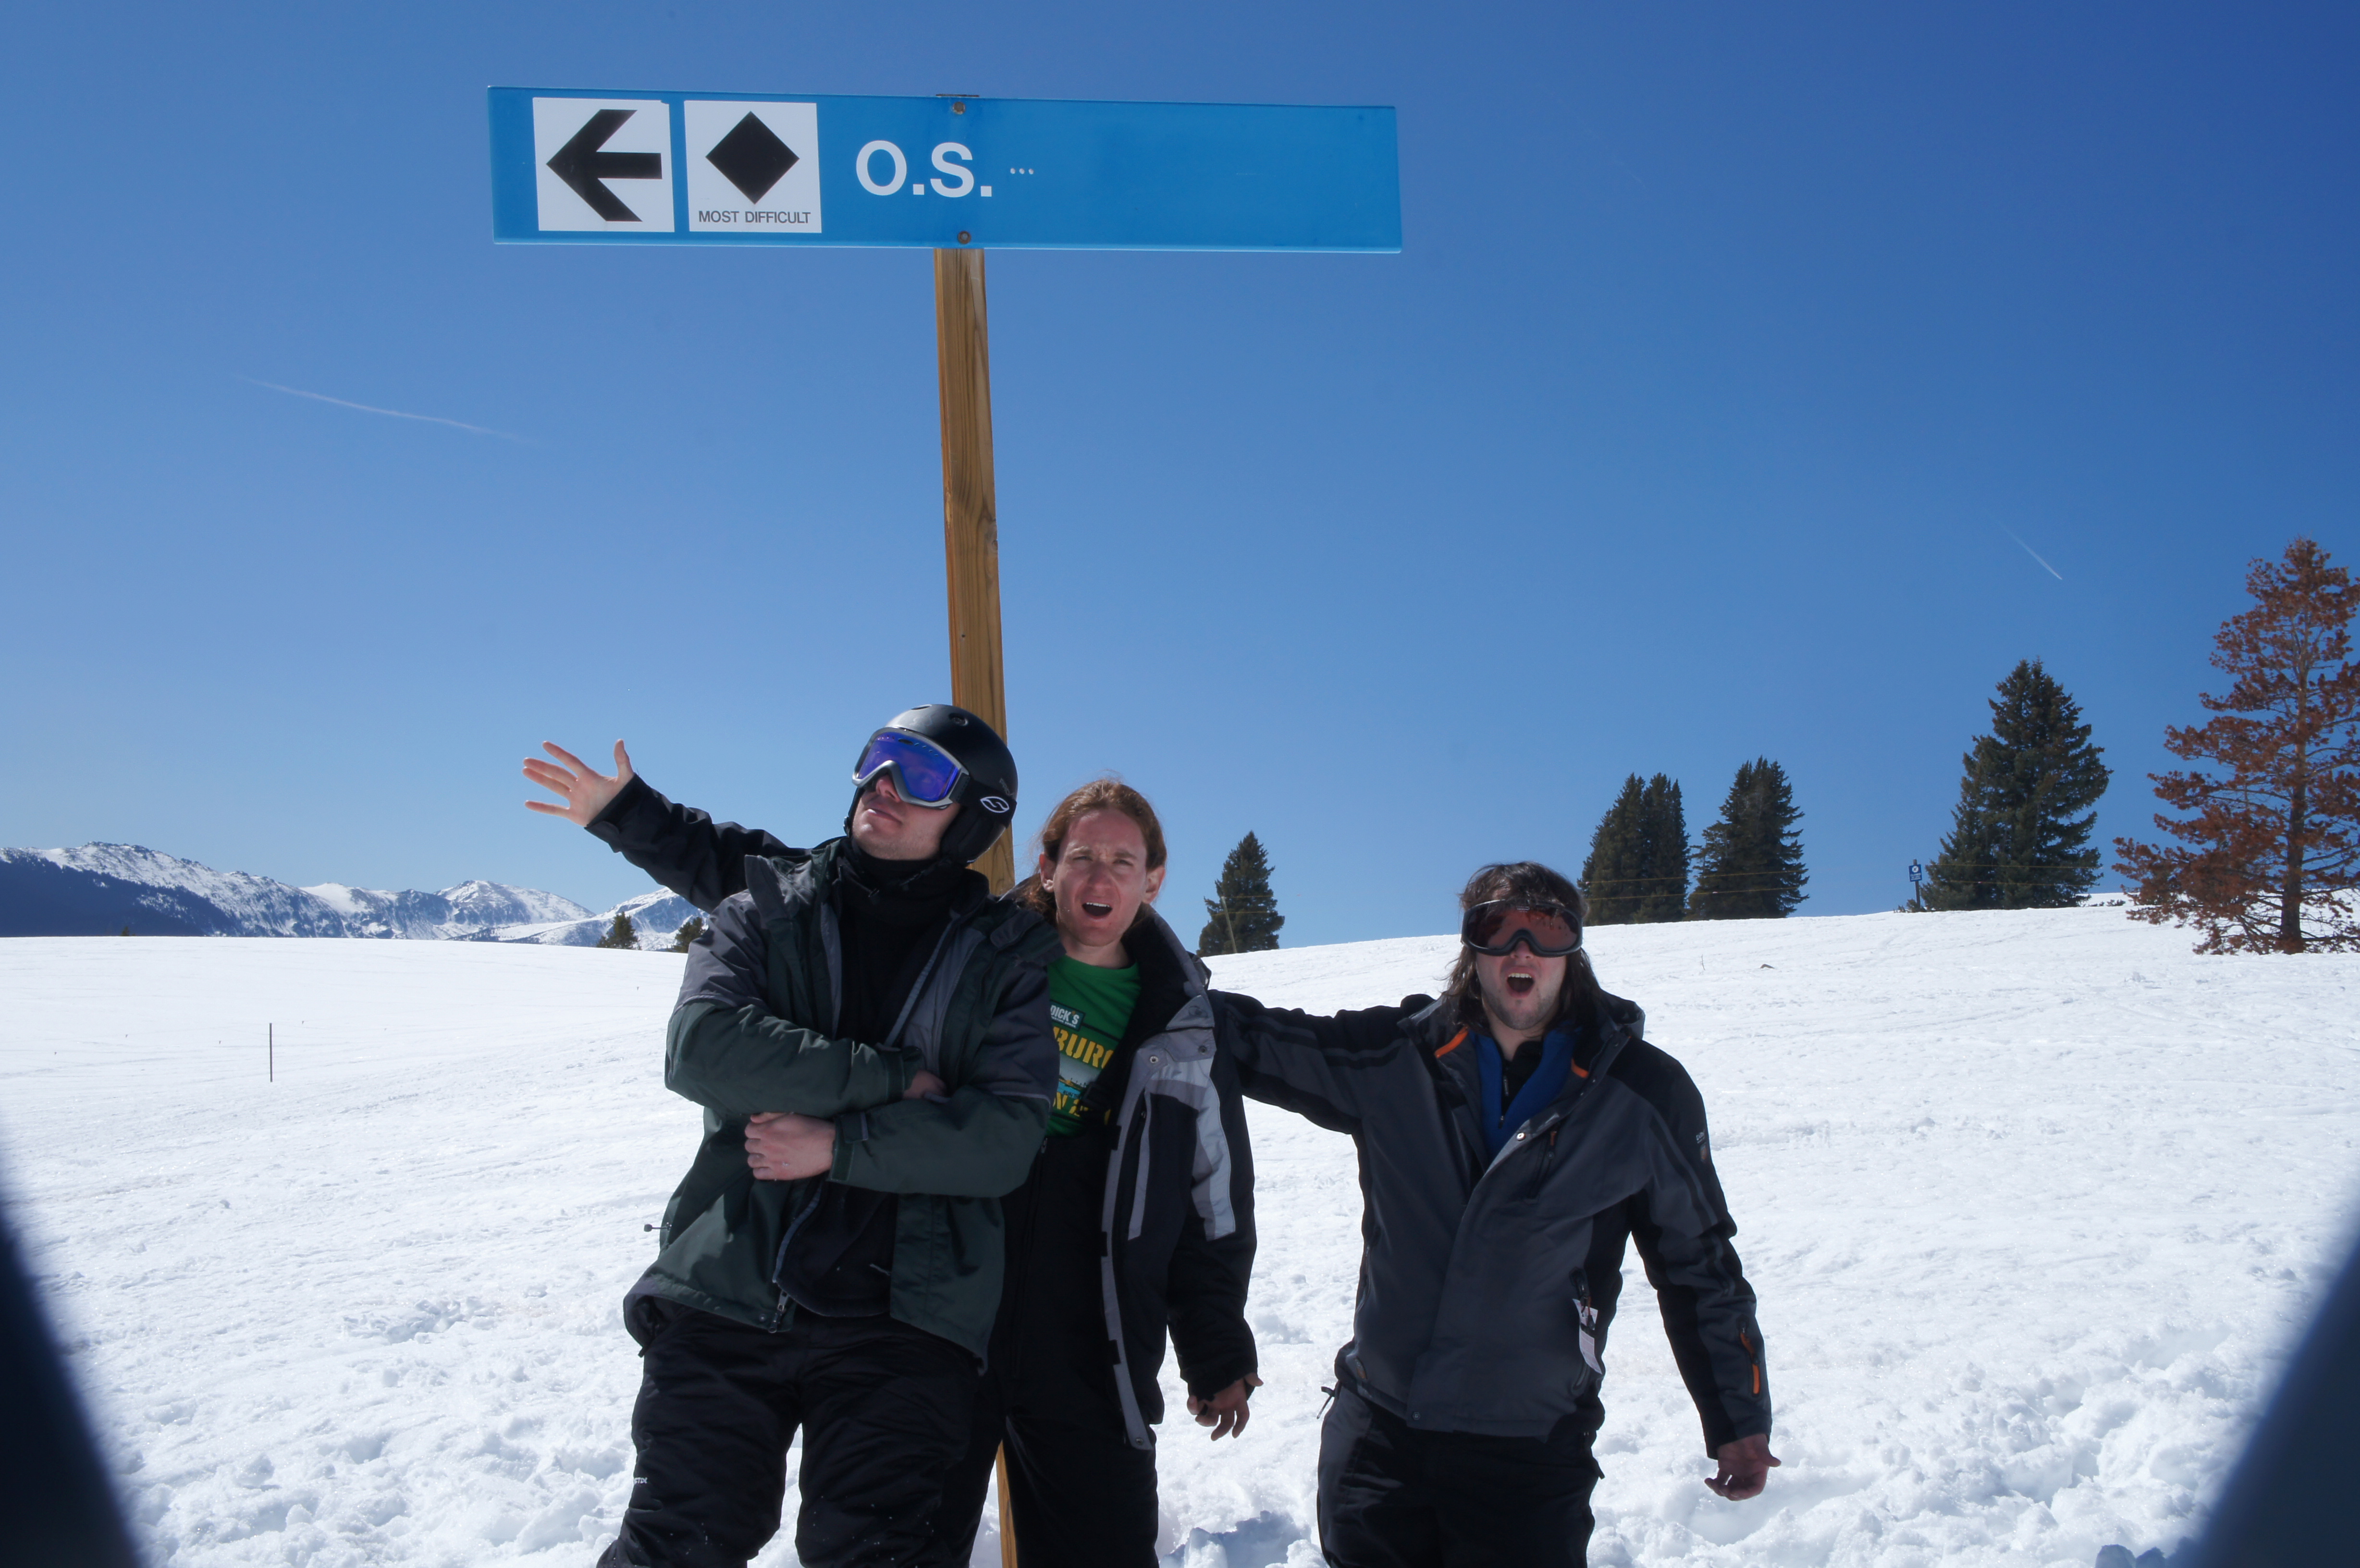
\includegraphics[width=0.75\textwidth]{wont-modify-vail.jpg}
	\end{center}
	\caption{Former members of Operating Systems course staff lament the difficulty involved in teaching students concurrency debugging skills.}
\end{figure*}

15-410 currently teaches students concurrency debugging skills ``the hard way'': by immersing them in environments where races will arise, and letting them find debugging tactics on their own to use in conjunction with conventional stress testing.

We believe that a tool such as Landslide could change the way students learn such skills for the better, beyond simply increasing their likelihood of finding bugs during testing. The decision tree is a much more structured way of expressing a test case's concurrent behaviour than the way 15-410 currently teaches, which is ``think hard until you figure out the buggy interleaving''. Having students use Landslide, even to a small extent, might encourage them to think in this more structured way.\footnote{
\revision{In 15-410, before the kernel project, students also implement a user-space thread library. Just as Landslide could help the students during the kernel project, so too could a user-space systematic exploration tool help during the thread library project.}}

\subsection{Landslide as a Grading Tool}

The 15-410 grading infrastructure currently uses a program called Fritz, which is a stress testing wrapper around a suite of test programs. Some of these tests are Landslide-friendly (Section~\ref{sec:using-landslide-friendly-tests}), and some are themselves stress tests. The 15-410 course staff also hand-grade every kernel, in part because Fritz is known for only catching race conditions at random and infrequently.

While far from being able to replace talented humans for grading, we believe that, after some improvement, Landslide could augment or replace Fritz as a tool for automatically finding several common patterns of concurrency errors that students have (especially races involving exiting threads, which we have shown Landslide is effective at finding).

%%%%%%%%%%%%%%%%%%%%%%%%%%%%%%%%%%%%%%%%%%%%%%%%%%%%%%%%%%%%%%%%%%%%%%%%%%%%%%%%
\section{New Techniques}
\label{sec:future-new}

Related research in dynamic verification has introduced testing techniques orthogonal to systematic exploration, which could augment its effectiveness if combined in one tool. We discuss the potential for using other techniques in Landslide or in any other systematic testing framework.

\subsection{Data Race Detection}
\label{sec:future-analysis}

Landslide currently never alters its set of decision points once it begins executing. The user must configure the set of decision points in advance, and Landslide follows them to the letter when exploring the tree. This is useful for investigating the size of trees generated by certain sets of decision points, but future work should do better than leaving it up to the user to stumble across a set of decision points that exposes a bug.

Most notably among the information Landslide has at its disposal is the collection of conflicting shared memory accesses among transitions. Theoretically, to identify a decision point immediately before and after each such access would generate an execution tree with perfect granularity (i.e., exactly one shared memory access per transition), and thence find every possible race condition - this is, of course, the opposite extreme to the current setup.

Landslide could make use of data race detection techniques\cite{datacollider}, however, to strike a middle ground in which shared memory accesses it chooses.
\begin{enumerate}
	\item It should be aware of the types and interfaces associated with the kernel's synchronisation primitives (mutexes, condvars, semaphores, etc), and be able to treat operations on those as ``guaranteed to work'' (similar to Section~\ref{sec:por-independence}).
	\item Next, it should recognise acquire and release (or sleep and wake) operations on synchronisation primitives, and use that information to track lockset-type information.
	\item Ultimately, it should use the lockset information in conjunction with the happens-before relation to identify which memory accesses are ``raciest'', and add decision points around those.
\end{enumerate}

\subsection{Parallelism}

Landslide's tree exploration is implemented sequentially. However, because DPOR's approach of tagging which sibling branches should be explored next generally follows a workqueue-based depth-first-search structure, it should not be too difficult to parallelise. Prior work exists for this technique\cite{distributed-dpor}, so it would not be a research contribution, but would substantially improve Landslide's effectiveness regardless.

\subsection{Symbolic Execution}

In Section~\ref{sec:related-orthogonal}, we mentioned the technique of symbolic execution for dynamic verification. We believe that symbolic execution could be combined with systematic exploration to help find races in certain obscure code paths that systematic exploration by itself might not even execute.

One interesting phenomenon that would occur from combining symbolic execution and systematic exploration would be a new notion of decision points. Symbolic execution involves its own state space exploration, in which control flow branch points correspond to decision points; hence, to combine it with systematic exploration would create a hybrid state space in which a ``decision point'' could be a place where either different threads could preempt each other or multiple control flow paths could be taken\cite{dawson}.

\subsection{Trace Minimisation}
\label{sec:future-trace-minimisation}

Also in Section~\ref{sec:related-orthogonal}, we mentioned related research that attempts to {\em minimise} the set of conditions that are known to be associated with a bug\cite{dag-mining}.
In the context of Landslide, this corresponds to how easy the decision trace is to understand. Even if Landslide finds a bug and prints the list of thread switches that were made, it may still be very difficult for the user to understand if the list includes many unnecessary switches that were completely unrelated to the bug.

Landslide could continue to be of use even after it has found a bug, by attempting to find a ``minimal decision trace''. It could search different subsets of the known-buggy trace in an attempt to find shorter traces which result in the same bug.
In this way, it would be able to print decision traces that automatically give the programmer much more insight into the true nature of each race condition.

While studying various bugs found by Landslide, we found that in general, when there were frivolous thread switches in the decision trace, users most benefitted from starting to read the trace at the end; i.e., considering the most recent transition made by each thread. Hence, when building a search algorithm for trace minimisation, it would be good to more heavily prioritise decisions that occurred later in a buggy branch.

%%%%%%%%%%%%%%%%%%%%%%%%%%%%%%%%%%%%%%%%%%%%%%%%%%%%%%%%%%%%%%%%%%%%%%%%%%%%%%%%
\section{Linux}
\label{sec:future-linux}

The Linux kernel is a logical next kernel architecture to target with Landslide.

One advantage of targetting Linux is that a testing framework will be able to make assumptions about the scheduler design, in ways that Landslide was not able to (Section~\ref{sec:challenges-design}), because the kernel instrumentation will not need to be repeatedly re-implemented (as it did for each 15-410 student kernel that we tested).

However, Linux is a much more complicated kernel architecture than Pebbles, and we would face several challenges.

\subsection{Multi-Processor Support}

Landslide's way of modelling concurrency as a tree of thread interleavings directly expresses the way concurrency arises on uniprocessor systems. On multiprocessor systems such as Linux, however, there is ``true concurrency'': different threads may be running at the same time on different processors, rather than just interleaved. Hence, race conditions that were previously impossible in a uniprocessor environment may be commonplace in SMP.

In order to support multiprocessor kernels, Landslide would need to refine its representation of the decision tree to express the potential for threads interleaving either on the same processor or on different processors. As a starting point, we note that on SMP, at each decision point, in addition to choosing any of $N$ threads to run, we must choose from among $M$ processors for it to run on.

\subsection{Performance}

Linux is much bigger than a Pebbles kernel (in terms of amount of code that runs during startup, during scheduling, etc), and hence would be much more expensive to test in a simulated environment. We suspect that in order to practically test Linux, we would need to implement systematic exploration in a virtualised environment, which we discuss more in Section~\ref{sec:future-virt}.

\subsection{Complicated Synchronisation Patterns}

Many components of Linux contain ad-hoc synchronisation which would be difficult to reason about. One common pattern is attempting some operation, checking later if it got interfered with, and rewinding and trying again if so. A straightforward approach to building a decision tree representing this might result in an infinitely deep branch: if the thread that gets interfered with keeps getting selected for scheduling, it would never make any progress. The testing tool would need to recognise these cases, and understand the invisible dependency on ``somebody else'' running first.

\subsection{Device Drivers}
\label{sec:future-drivers}

There is much more device driver code in Linux than there is for its core components, and the device driver code also does not undergo as rigorous code review. Because of this, device drivers are much more prone to concurrency errors than the core components, and hence a systematic exploration framework for Linux should focus on testing them.

However, the concurrency model of device drivers is much more complicated than the simple timer-based scheduling model we used in this work. In addition to timer-driven preemptions, code may also be interleaved as caused by device interrupts and input. Like support for SMP, being able to systematically test for device driver races will also require a more sophisticated representation of the decision tree.

In addition to controlling timer interrupts, a systematic testing tool would also need to control device interrupts and device input, both of which are also nondeterministic inputs to the kernel. Furthermore, it would need to recognise common components of device drivers to properly cause relevant scheduling patterns, such as the ``top half'' and ``bottom half'' of interrupt handlers and dedicated device driver threads.

These components would all be candidates for being scheduled at a decision point, although it more complicated still than simply choosing from among several threads to run. For example, the bottom half of an interrupt handler would depend on a top half having already executed, and interrupt handlers would run on the same stack as other thread rather than on their own stack.

% FIXME
%\subsection{Other Kernel Environments}

%Some other production kernels would also make good targets for systematic exploration.

%%%%%%%%%%%%%%%%%%%%%%%%%%%%%%%%%%%%%%%%%%%%%%%%%%%%%%%%%%%%%%%%%%%%%%%%%%%%%%%%
\section{Virtualisation}
\label{sec:future-virt}

Compared to executing the code being tested on real hardware (which tools such as \cite{dbug-ssv} are able to do for user-space programs), Simics is {\em slow}, and even slower with Landslide hooked up to it.

Major benefit could be achieved by redesigning Landslide to work in a virtualised environment instead of a simulated one. This would pose several challenges, because Landslide would no longer be running in ``god mode'', having immediate access to every single instruction and memory access executed. It would, however, still be able to modify the kernel's memory and address space, which would be important to harness for increased control over the kernel's execution.

We speculate on some challenges and potential solutions that virtualised execution might have to offer. We assume that our users will be talented kernel developers rather than undergraduate students, and hence allow for more complicated interface requirements.

\subsection{Interposition}

\subsubsection{Event Tracking}

The event-based nature of the \texttt{tell\_landslide} annotations can still be harnessed in a virtualised environment - they would need to be converted into hypercalls, which would briefly transfer control to Landslide at key execution points to enable it to update its state machine and potentially influence the kernel's execution.

We would add additional \texttt{tells\_landslide} for the kernel components which are presently automatically instrumented, such as the dynamic memory allocator and the \texttt{panic} routines, and also for certain components that are currently instrumented with \texttt{config.landslide}, such as identifying when the context switcher returns or when the timer interrupt handler is invoked.

Rather than using the schedule-in-flight algorithm, Landslide could simplify its job by asking the kernel to run a particular thread directly, as described in Section~\ref{sec:components-inflight}.

\subsubsection{Memory Tracking}

More challenging than tracking important kernel events will be tracking all accesses to shared memory. We could exploit the virtualised virtual memory system, and write-protect (possibly also read-protect, i.e., unmap) all pages that contain shared data, such as the global data section and the dynamic allocation heap. All accesses would then page-fault, transferring control to Landslide.

\subsection{Backtracking}

Simics's convenient bookmarking mechanism will be no more in virtual-machine-land. One possibility for backtracking would be to record-and-replay the events of each branch (up to the point at which Landslide chooses to have decided differently), restarting the system's execution from the beginning each time. Another option might be to snapshot the state of the kernel at each decision point, and use those to resume without re-executing everything from the beginning (kernel boot-up and initialisation is much more expensive than individual system calls, after all).

\subsection{Control over Non-Determinism}

Finally, Landslide will need to find new ways to control non-deterministic events in the system. Since virtualised kernels use the same timer interrupt as the host they run on, Landslide is unlikely to be able to intercept it. Instead, we may replace a guest kernel's timer-driven context switcher with a ``Landslide-driven'' context switcher, leaving the timer handler only to do other work.

Likewise, Landslide will need to control other non-deterministic inputs to the kernel, including device interrupts/input and even the system clock.

%%%%%%%%%%%%%%%%%%%%%%%%%%%%%%%%%%%%%%%%%%%%%%%%%%%%%%%%%%%%%%%%%%%%%%%%%%%%%%%%
\section{Long-Running Test Shaping}
\label{sec:future-shaping}

Another area to investigate is that of systems which could be tested continuously. Instead of the goal of finishing exploring a test case without finding a bug, a long-running testing approach would focus on ``shaping'' the test configuration to more and more refined configurations in hopes of finding a bug eventually.

%\subsection{Iterating Decision Sets}
In Section~\ref{sec:discussion-strategies}, we recommend an iteration strategy to effectively explore trees with multiple different sets of decision points, while not knowing ahead of time which, if any, may contain a bug.
This strategy would give rise to a test framework which could explore multiple different types and granularities of interleavings at once, heuristically judge which are more likely to uncover bugs, and prioritise resource allocation and search direction accordingly.

There is also the question of when during the testing process new decision points should be introduced.
One possibility would be to begin exploration with a small set of decision points, explore the resulting tree, analyse the tree post-hoc to identify additional decision points, and iterate exploring with the new set.
Another possibility would be to identify decision points along the way, analysing each branch of the tree after executing it, to generate the decision points for that very branch, and thence use them to find which branch to explore next.
It remains to be seen which approach would be more effective.

% TODO talk about heuristic-guided tree construction

% FIXME
%In Section~\ref{Sec:future-nadim}, we discuss an interesting property of certain decision trees, and suggest a heuristic

%%%%%%%%%%%%%%%%%%%%%%%%%%%%%%%%%%%%%%%%%%%%%%%%%%%%%%%%%%%%%%%%%%%%%%%%%%%%%%%%
\section{Theoretical Oddities}
\label{sec:future-theory}

During our in-depth case studies, we noticed two interesting properties about certain decision trees. We believe these warrant further theoretical study, to better understand the nature of these decision trees. This may in turn give rise to heuristics for making systematic testing more effective.

% TODO: make visualisations for both of these
\subsection{``Backwards'' Exploration}
\label{sec:future-backwards}

We configured Landslide to be able to explore trees in two different orderings, and we found that the two orderings behaved substantially differently in terms of time taken to find bugs and length of decision traces produced.

\begin{itemize}
	\item {\bf Forwards exploration.} When exploring the tree ``forwards'', at each decision point the explorer would choose the currently-running thread if it hadn't already been explored. This resulted in preference for branches of the tree with fewer forced preemptions; the first branch to be explored would have no preemptions at all, and subsequent branches would have generally (but not monotonically) increasing numbers of preemptions.

		Compared to backwards exploration, we found that forwards exploration tended to produce much shorter decision traces for the same bugs. These shorter traces would have fewer thread switches that were irrelevant to the bug itself, and hence be much easier to understand.
	\item {\bf Backwards exploration.} When exploring ``backwards'', at each decision point the explorer would prefer to choose a thread that required a forced preemption. This resulted in preference for branches with more forced preemptions, and the first branch to be explored would have a preemption at every decision point.\footnote{
		This property of backwards exploration is what resulted in the LudicrOS yield/vanish bug being found without any backtracks.}

		Compared to forwards exploration, we found that backwards exploration tended to find bugs much more quickly, with fewer backtracks needed before the buggy branch was chosen.
\end{itemize}
% TODO: provide results here
% FIXME: study diffs in trees with no bugs at all

Compared to Iterative Context Bounding\cite{chess}, which is based on the insight that bugs need fewer forced preemptions to expose, we believe that our insight is orthogonal. The ICB insight results in smaller decision trees overall needing to be explored before bugs appear, while our insight determines exploration ordering once the tree is constructed.

We are not sure if combining these two insights is possible. In future work we might compare them and investigate this possibility, to determine a heuristic for what exploration orderings are most likely to expose bugs with the fewest needed preemptions.

\subsection{Exploration Tree Structure}
\label{sec:future-nadim}

One member of group 1 from the user study fully explored decision trees from \texttt{double\_wait} and \texttt{vanish\_vanish} (Section~\ref{sec:eval-victory}), and found an oddity in the exploration time for a particular decision set.

When using decision points on just \texttt{mutex\_lock} or \texttt{mutex\_unlock}, the explorations for each test case took similar time. However, when using decision points on both mutex functions, \texttt{double\_wait} took substantially longer, despite the tree structure suggesting they should have been comparable, with \texttt{double\_wait} even being perhaps slightly faster. Figure~\ref{fig:nadim-stats} shows a comparison of the tree anatomy for these two test cases.

\begin{figure}[h]
	\small
	\centering
	\begin{tabular}{|l||c|c|}
		\hline
		& \texttt{double\_wait} & \texttt{vanish\_vanish} \\
		\hline\hline
		Exploration time & {\bf 30 minutes} & {\bf 5 minutes} \\
		\hline
		Backtracks & {\bf 1,401} & {\bf 1,511} \\
		\hline
		Decision points & 10,355 & 5,690 \\
		\hline
		Average branch depth & 18.34 & 16.00 \\
		\hline
		Average instructions/branch& 1,975,033 & 1,984,249 \\
		\hline
		Total instructions & 206,757,601 & 24,907,516 \\
		\hline
		Backtrack distance minimum & {\bf 6} & {\bf 2} \\
		\hline
		Backtrack distance maximum & 17 & 16 \\
		\hline
		Backtrack distance average & {\bf 7.38}  & {\bf 3.75} \\
		\hline
		% FIXME: add stddev?
	\end{tabular}
	\caption{Comparison of expensive \texttt{double\_wait} test and cheap \texttt{vanish\_vanish} test. The number of branches and depth of each branch are similar, but \texttt{double\_wait}'s backtracks were significantly longer, causing more total instructions to be executed.}
	\label{fig:nadim-stats}
\end{figure}

Despite the two trees having nearly equal numbers of branches and instructions executed per branch, \texttt{double\_wait} took significantly more time. This is because Landslide's backtracks during \texttt{double\_wait} were significantly {\em longer} than the backtracks in \texttt{vanish\_vanish} on average; i.e., the backtracks were targetting an earlier point during the test's execution.
Hence, Landslide had to execute more total instructions overall to explore the longer branches in \texttt{double\_wait}.\footnote{
Of note, if backtracking had been implemented by restarting the test each time; i.e., executing the full depth of every branch from the root of the tree, the repeated work would have caused the execution times to be equal. The fact that Simics's backtracking avoids the cost of execution that happened before the backtrack target is to credit for this discrepancy.}
% as visualised in figure\ldots TODO

This suggests that the ``interesting'' parts of \texttt{double\_wait} were earlier in the test case, whereas in \texttt{vanish\_vanish} they are more towards the end. We conjecture that, with theoretical study of these structural properties, we could develop search heuristics for focusing on the ``interesting'' parts of the trees, and avoid repeating the irrelevant instructions at the end of each branch.
